\documentclass[journal,12pt,twocolumn]{IEEEtran}
%
\usepackage{setspace}
\usepackage{gensymb}
%\doublespacing
\singlespacing

%\usepackage{graphicx}
%\usepackage{amssymb}
%\usepackage{relsize}
\usepackage[cmex10]{amsmath}
%\usepackage{amsthm}
%\interdisplaylinepenalty=2500
%\savesymbol{iint}
%\usepackage{txfonts}
%\restoresymbol{TXF}{iint}
%\usepackage{wasysym}
\usepackage{amsthm}
\usepackage{iithtlc}
\usepackage{mathrsfs}
\usepackage{txfonts}
\usepackage{stfloats}
\usepackage{bm}
\usepackage{cite}
\usepackage{cases}
\usepackage{subfig}
%\usepackage{xtab}
\usepackage{longtable}
\usepackage{multirow}
%\usepackage{algorithm}
%\usepackage{algpseudocode}
\usepackage{enumitem}
\usepackage{mathtools}
\usepackage{tikz}
\usepackage{circuitikz}
\usepackage{verbatim}
\usepackage{tfrupee}
\usepackage[breaklinks=true]{hyperref}
%\usepackage{stmaryrd}
\usepackage{tkz-euclide} % loads  TikZ and tkz-base
\usetkzobj{all}
\usetikzlibrary{fit}
\pgfdeclarelayer{background}
\pgfsetlayers{background}
\usepackage{listings}
    \usepackage{color}                                            %%
    \usepackage{array}                                            %%
    \usepackage{longtable}                                        %%
    \usepackage{calc}                                             %%
    \usepackage{multirow}                                         %%
    \usepackage{hhline}                                           %%
    \usepackage{ifthen}                                           %%
  %optionally (for landscape tables embedded in another document): %%
    \usepackage{lscape}     
\usepackage{multicol}
\usepackage{chngcntr}
%\usepackage{enumerate}

%\usepackage{wasysym}
%\newcounter{MYtempeqncnt}
\DeclareMathOperator*{\Res}{Res}
%\renewcommand{\baselinestretch}{2}
\renewcommand\thesection{\arabic{section}}
\renewcommand\thesubsection{\thesection.\arabic{subsection}}
\renewcommand\thesubsubsection{\thesubsection.\arabic{subsubsection}}

\renewcommand\thesectiondis{\arabic{section}}
\renewcommand\thesubsectiondis{\thesectiondis.\arabic{subsection}}
\renewcommand\thesubsubsectiondis{\thesubsectiondis.\arabic{subsubsection}}

% correct bad hyphenation here
\hyphenation{op-tical net-works semi-conduc-tor}
\def\inputGnumericTable{}                                 %%

\lstset{
%language=C,
frame=single, 
breaklines=true,
columns=fullflexible
}
%\lstset{
%language=tex,
%frame=single, 
%breaklines=true
%}

\begin{document}
%


\newtheorem{theorem}{Theorem}[section]
\newtheorem{problem}{Problem}
\newtheorem{proposition}{Proposition}[section]
\newtheorem{lemma}{Lemma}[section]
\newtheorem{corollary}[theorem]{Corollary}
\newtheorem{example}{Example}[section]
\newtheorem{definition}[problem]{Definition}
%\newtheorem{thm}{Theorem}[section] 
%\newtheorem{defn}[thm]{Definition}
%\newtheorem{algorithm}{Algorithm}[section]
%\newtheorem{cor}{Corollary}
\newcommand{\BEQA}{\begin{eqnarray}}
\newcommand{\EEQA}{\end{eqnarray}}
\newcommand{\define}{\stackrel{\triangle}{=}}

\bibliographystyle{IEEEtran}
%\bibliographystyle{ieeetr}


\providecommand{\mbf}{\mathbf}
\providecommand{\pr}[1]{\ensuremath{\Pr\left(#1\right)}}
\providecommand{\qfunc}[1]{\ensuremath{Q\left(#1\right)}}
\providecommand{\sbrak}[1]{\ensuremath{{}\left[#1\right]}}
\providecommand{\lsbrak}[1]{\ensuremath{{}\left[#1\right.}}
\providecommand{\rsbrak}[1]{\ensuremath{{}\left.#1\right]}}
\providecommand{\brak}[1]{\ensuremath{\left(#1\right)}}
\providecommand{\lbrak}[1]{\ensuremath{\left(#1\right.}}
\providecommand{\rbrak}[1]{\ensuremath{\left.#1\right)}}
\providecommand{\cbrak}[1]{\ensuremath{\left\{#1\right\}}}
\providecommand{\lcbrak}[1]{\ensuremath{\left\{#1\right.}}
\providecommand{\rcbrak}[1]{\ensuremath{\left.#1\right\}}}
\theoremstyle{remark}
\newtheorem{rem}{Remark}
\newcommand{\sgn}{\mathop{\mathrm{sgn}}}
\providecommand{\abs}[1]{\left\vert#1\right\vert}
\providecommand{\res}[1]{\Res\displaylimits_{#1}} 
\providecommand{\norm}[1]{\left\lVert#1\right\rVert}
%\providecommand{\norm}[1]{\lVert#1\rVert}
\providecommand{\mtx}[1]{\mathbf{#1}}
\providecommand{\mean}[1]{E\left[ #1 \right]}
\providecommand{\fourier}{\overset{\mathcal{F}}{ \rightleftharpoons}}
%\providecommand{\hilbert}{\overset{\mathcal{H}}{ \rightleftharpoons}}
\providecommand{\system}{\overset{\mathcal{H}}{ \longleftrightarrow}}
	%\newcommand{\solution}[2]{\textbf{Solution:}{#1}}
\newcommand{\solution}{\noindent \textbf{Solution: }}
\newcommand{\cosec}{\,\text{cosec}\,}
\providecommand{\dec}[2]{\ensuremath{\overset{#1}{\underset{#2}{\gtrless}}}}
\newcommand{\myvec}[1]{\ensuremath{\begin{pmatrix}#1\end{pmatrix}}}
\newcommand{\mydet}[1]{\ensuremath{\begin{vmatrix}#1\end{vmatrix}}}
%\numberwithin{equation}{section}
\numberwithin{equation}{subsection}
%\numberwithin{problem}{section}
%\numberwithin{definition}{section}
\makeatletter
\@addtoreset{figure}{problem}
\makeatother

\let\StandardTheFigure\thefigure
\let\vec\mathbf
%\renewcommand{\thefigure}{\theproblem.\arabic{figure}}
\renewcommand{\thefigure}{\theproblem}
%\setlist[enumerate,1]{before=\renewcommand\theequation{\theenumi.\arabic{equation}}
%\counterwithin{equation}{enumi}


%\renewcommand{\theequation}{\arabic{subsection}.\arabic{equation}}

\def\putbox#1#2#3{\makebox[0in][l]{\makebox[#1][l]{}\raisebox{\baselineskip}[0in][0in]{\raisebox{#2}[0in][0in]{#3}}}}
     \def\rightbox#1{\makebox[0in][r]{#1}}
     \def\centbox#1{\makebox[0in]{#1}}
     \def\topbox#1{\raisebox{-\baselineskip}[0in][0in]{#1}}
     \def\midbox#1{\raisebox{-0.5\baselineskip}[0in][0in]{#1}}

\vspace{3cm}

\title{
	\logo{
Discrete Maths and Algebra
	}
}
\author{ G V V Sharma$^{*}$% <-this % stops a space
	\thanks{*The author is with the Department
		of Electrical Engineering, Indian Institute of Technology, Hyderabad
		502285 India e-mail:  gadepall@iith.ac.in. All content in this manual is released under GNU GPL.  Free and open source.}
	
}	
%\title{
%	\logo{Matrix Analysis through Octave}{\begin{center}
\includegraphics[scale=.24]{tlc}\end{center}}{}{HAMDSP}
%}


% paper title
% can use linebreaks \\ within to get better formatting as desired
%\title{Matrix Analysis through Octave}
%
%
% author names and IEEE memberships
% note positions of commas and nonbreaking spaces ( ~ ) LaTeX will not break
% a structure at a ~ so this keeps an author's name from being broken across
% two lines.
% use \thanks{} to gain access to the first footnote area
% a separate \thanks must be used for each paragraph as LaTeX2e's \thanks
% was not built to handle multiple paragraphs
%

%\author{<-this % stops a space
%\thanks{}}
%}
% note the % following the last \IEEEmembership and also \thanks - 
% these prevent an unwanted space from occurring between the last author name
% and the end of the author line. i.e., if you had this:
% 
% \author{....lastname \thanks{...} \thanks{...} }
%                     ^------------^------------^----Do not want these spaces!
%
% a space would be appended to the last name and could cause every name on that
% line to be shifted left slightly. This is one of those "LaTeX things". For
% instance, "\textbf{A} \textbf{B}" will typeset as "A B" not "AB". To get
% "AB" then you have to do: "\textbf{A}\textbf{B}"
% \thanks is no different in this regard, so shield the last } of each \thanks
% that ends a line with a % and do not let a space in before the next \thanks.
% Spaces after \IEEEmembership other than the last one are OK (and needed) as
% you are supposed to have spaces between the names. For what it is worth,
% this is a minor point as most people would not even notice if the said evil
% space somehow managed to creep in.



% The paper headers
%\markboth{Journal of \LaTeX\ Class Files,~Vol.~6, No.~1, January~2007}%
%{Shell \MakeLowercase{\textit{et al.}}: Bare Demo of IEEEtran.cls for Journals}
% The only time the second header will appear is for the odd numbered pages
% after the title page when using the twoside option.
% 
% *** Note that you probably will NOT want to include the author's ***
% *** name in the headers of peer review papers.                   ***
% You can use \ifCLASSOPTIONpeerreview for conditional compilation here if
% you desire.




% If you want to put a publisher's ID mark on the page you can do it like
% this:
%\IEEEpubid{0000--0000/00\$00.00~\copyright~2007 IEEE}
% Remember, if you use this you must call \IEEEpubidadjcol in the second
% column for its text to clear the IEEEpubid mark.



% make the title area
\maketitle

\newpage

\tableofcontents

\bigskip

\renewcommand{\thefigure}{\theenumi}
\renewcommand{\thetable}{\theenumi}
%\renewcommand{\theequation}{\theenumi}

%\begin{abstract}
%%\boldmath
%In this letter, an algorithm for evaluating the exact analytical bit error rate  (BER)  for the piecewise linear (PL) combiner for  multiple relays is presented. Previous results were available only for upto three relays. The algorithm is unique in the sense that  the actual mathematical expressions, that are prohibitively large, need not be explicitly obtained. The diversity gain due to multiple relays is shown through plots of the analytical BER, well supported by simulations. 
%
%\end{abstract}
% IEEEtran.cls defaults to using nonbold math in the Abstract.
% This preserves the distinction between vectors and scalars. However,
% if the journal you are submitting to favors bold math in the abstract,
% then you can use LaTeX's standard command \boldmath at the very start
% of the abstract to achieve this. Many IEEE journals frown on math
% in the abstract anyway.

% Note that keywords are not normally used for peerreview papers.
%\begin{IEEEkeywords}
%Cooperative diversity, decode and forward, piecewise linear
%\end{IEEEkeywords}



% For peer review papers, you can put extra information on the cover
% page as needed:
% \ifCLASSOPTIONpeerreview
% \begin{center} \bfseries EDICS Category: 3-BBND \end{center}
% \fi
%
% For peerreview papers, this IEEEtran command inserts a page break and
% creates the second title. It will be ignored for other modes.
%\IEEEpeerreviewmaketitle

\begin{abstract}
This book provides a computational approach to school algebra and discrete mathematics based on the NCERT textbooks from Class 6-12.  Links to sample Python codes are available in the text.  
\end{abstract}
Download python codes using 
\begin{lstlisting}
svn co https://github.com/gadepall/school/trunk/ncert/codes
\end{lstlisting}

\section{Probability}
\subsection{Examples}
\renewcommand{\theequation}{\theenumi}
\begin{enumerate}[label=\arabic*.,ref=\thesubsection.\theenumi]
\numberwithin{equation}{enumi}
\item If P(A)=$\frac{7}{13}, P(B)=\frac{9}{13}$ and $P(A\cap B)=\frac{4}{13},$ Evaluate P(A/B)?\\

\item A family has two children. What is the probability that both the children are boys given that at least one of them is a boy?\\

\item Ten cards numbered 1 to 10 are placed in a box, mixed up thoroughly and then one card is drawn randomly. If it is known that the number on the drawn card is more than 3, what is the probability that it is an even number?\\

\item In a school, there are 1000 students, out of which 430 are girls. It is known that out of 430,  10 percentage of the girls study in class XII. What is the probability that a student chosen randomly studies in Class XII given that the chosen student is a girl?\\

\item A die is thrown three times. Events A and B are defined as below:\\
A : 4 on the third throw.\\
B : 6 on the first and 5 on the second throw.\\
Find the probability of A given that B has already occurred?\\

\item A die is thrown twice and the sum of the numbers appearing is observed to be 6. What is the conditional probability that the number 4 has appeared at least once?\\

\item Consider the experiment of tossing a coin. If the coin shows head, toss it again but if it shows tail, then throw a die. Find the conditional probability of the event that "the die shows a number greater than 4" given that "there is at least one tail".\\

\item An urn contains 10 black and 5 white balls. Two balls are drawn from the urn one after the other without replacement. What is the probability that both drawn balls are black?\\

\item Three cards are drawn successively, without replacement from a pack of 52 well shuffled cards. What is the probability that first two cards are kings and the third card drawn is an ace?\\

\item A die is thrown. If E is the event "the number appearing is a multiple of 3" and F be the event "the number appearing is even" then find whether E and F are independent ?\\

\item An unbiased die is thrown twice. Let the event A be "odd number on the first throw" and B the event "odd number on the second throw". Check the independence of the events A and B.\\

\item Three coins are tossed simultaneously. Consider the event E "three heads or three tails", F "at least two heads" and G "at most two heads". Of the pairs (E,F), (E,G) and (F,G), which are independent? which are dependent?\\

\item Prove that if E and F are independent events, then so are the events E and $F^{'}$.\\

\item If A and B are two independent events, then the probability of occurrence of at least one of A and B is given by 1- $P(A^{'}) P(B^{'})$\\

\item A person has undertaken a construction job. The probabilities are 0.65 that there will be strike, 0.80 that the construction job will be completed on time if there is no strike, and 0.32 that the construction job will be completed on time if there is a strike. Determine the probability that the construction job will be completed on time.\\

\item Bag I contains 3 red and 4 black balls while another Bag II contains 5 red and 6 black balls. One ball is drawn at random from one of the bags and it is found to be red. Find the probability that it was drawn from Bag II.\\

\item Given three identical boxes I, II and III, each containing two coins. In box I, both coins are gold coins, in box II, both are silver coins and in the box III, there is one gold and one silver coin. A person chooses a box at random and takes out a coin. If the coin is of gold, what is the probability that the other coin in the box is also of gold?\\

\item Suppose that the reliability of a HIV test is specified as follows: Of people having HIV, 90$\%$ of the test detect the disease but 10$\%$ go undetected. Of people free of HIV, 99$\%$ of the test are judged HIV –ve but 1$\%$ are diagnosed as showing HIV +ve. From a large population of which only 0.1$\%$ have HIV, one person is selected at random, given the HIV test, and the pathologist reports him/her as HIV +ve. What is the probability that the person actually has HIV?\\

\item In a factory which manufactures bolts, machines A, B and C manufacture respectively 25$\%$, 35$\%$ and 40$\%$ of the bolts. Of their outputs, 5, 4 and 2 percent are respectively defective bolts. A bolt is drawn at random from the product and is found to be defective. What is the probability that it is manufactured by the machine B?\\

\item A doctor is to visit a patient. From the past experience, it is known that the probabilities that he will come by train, bus, scooter or by other means of transport are respectively $\frac{3}{10},\frac{1}{5},\frac{1}{10}$ and $\frac{2}{5}.$ The probabilities that he will be late are $\frac{1}{4},\frac{1}{3}$ and $\frac{1}{12},$ if he comes by train, bus and scooter respectively, but if he comes by other means of transport, then he will not be late. When he arrives, he is late. What is the probability that he comes by train?\\

\item A man is known to speak truth 3 out of 4 times. He throws a die and reports that it is a six. Find the probability that it is actually a six.\\

\item A person plays a game of tossing a coin thrice. For each head, he is given Rs 2 by the organiser of the game and for each tail, he has to give Rs 1.50 to the organiser. Let X denote the amount gained or lost by the person. Show that X is a random variable and exhibit it as a function on the sample space of the experiment.\\

\item A bag contains 2 white and 1 red balls. One ball is drawn at random and then put back in the box after noting its colour. The process is repeated again. If X denotes the number of red balls recorded in the two draws, describe X.\\

\item Two cards are drawn successively with replacement from a well shuffled deck of 52 cards. Find the probability distribution of the number of aces.\\

\item Find the probability distribution of number of doublets in three throws of a pair of dice?\\

\item Let X denote the number of hours you study during a randomly selected school day. The probability that X can take the values x, has the following form, where k is some unknown constant.\\
P(X=x)= $\begin{pmatrix} 0.1, if x= 0 \\ kx,if x= 1 or 2 \\ k(5-x), if x= 3 or 4 \\ 0, otherwise \end{pmatrix}$\\
(a) Find the value of k.\\
(b) What is the probability that you study at least two hours ? Exactly two hours? At
most two hours?\\

\item Let a pair of dice be thrown and the random variable X be the sum of the numbers that appear on the two dice. Find the mean or expectation of X.\\

\item Find the variance of the number obtained on a throw of an unbiased die.\\

\item Two cards are drawn simultaneously (or successively without replacement) from a well shuffled pack of 52 cards. Find the mean, variance and standard deviation of the number of kings.\\

\item Six balls are drawn successively from an urn containing 7 red and 9 black balls. Tell whether or not the trials of drawing balls are Bernoulli trials when after each draw the ball drawn is\\
(i) replaced \\
(ii) not replaced in the urn.\\

\item If a fair coin is tossed 10 times, find the probability of\\
(i) exactly six heads\\
(ii) at least six heads\\
(iii) at most six heads\\

\item Ten eggs are drawn successively with replacement from a lot containing 10$\%$ defective eggs. Find the probability that there is at least one defective egg.\\

\item Coloured balls are distributed in four boxes as shown in the following table:\\
\\$\begin{tabular}{||c c c c c||} 
 \hline
 Box & Black & White & Red & Blue \\
 \hline\hline
 I & 3 & 4 & 5 & 6 \\
 \hline
 II & 2 & 2 & 2 & 2 \\
 \hline
 III & 1 & 2 & 3 & 1 \\
 \hline
 IV & 4 & 3 & 1 & 5 \\
 \hline
\end{tabular}$\\
\\A box is selected at random and then a ball is randomly drawn from the selected box. The colour of the ball is black, what is the probability that ball drawn is from the box III?\\

\item Find the mean of the Binomial distribution B(4,$\frac{1}{3}$).\\

\item The probability of a shooter hitting a target is $\frac{3}{4}$. How many minimum
number of times must he/she fire so that the probability of hitting the target at least
once is more than 0.99?\\

\item A and B throw a die alternatively till one of them gets a '6' and wins the game. Find their respective probabilities of winning, if A starts first.\\

\item If a machine is correctly set up, it produces 90$\%$ acceptable items. If it is
incorrectly set up, it produces only 40$\%$ acceptable items. Past experience shows that
80$\%$ of the set ups are correctly done. If after a certain set up, the machine produces 2 acceptable items, find the probability that the machine is correctly setup.\\
\item Find the probability of getting a head when a coin is tossed once. Also
find the probability of getting a tail.
\item A bag contains a red ball, a blue ball and a yellow ball, all the balls being
of the same size.Kritika takes out a ball from the bag without looking into it. What is the probability that she takes out the
(i) yellow ball? \\
(ii) red ball?\\
(iii) blue ball?
\item Suppose we throw a die once. (i) What is the probability of getting a number greater than 4 ? (ii) What is the probability of getting a number less than or
equal to 4 ?
\item One card is drawn from a well-shuffled deck of 52 cards. Calculate the
probability that the card will\\
(i) be an ace,\\
(ii) not be an ace.
\item Two players, Sangeeta and Reshma, play a tennis match. It is known
that the probability of Sangeeta winning the match is 0.62. What is the probability of
Reshma winning the match?
\item Savita and Hamida are friends. What is the probability that both will have \\
(i) different birthdays? \\
(ii) the same birthday? (ignoring a leap year).
\item There are 40 students in Class X of a school of whom 25 are girls and 15 are boys. The class teacher has to select one student as a class representative. She writes the name of each student on a separate card, the cards being identical.Then
she puts cards in a bag and stirs them thoroughly. She then draws one card from the
bag. What is the probability that the name written on the card is the name of\\
(i) a girl?\\
(ii) a boy?
\item  A box contains 3 blue, 2 white, and 4 red marbles. If a marble is drawn
at random from the box, what is the probability that it will be
(i) white? (ii) blue? (iii) red?
\item Harpreet tosses two different coins simultaneously (say, one is of rupee 1
and other of rupee 2). What is the probability that she gets at least one head?
\item In a musical chair game, the person playing the music has been
advised to stop playing the music at any time within 2 minutes after she starts playing.What is the probability that the music will stop within the first half-minute after starting?
\item A missing helicopter is reported to have crashed somewhere in the rectangular region shown in Fig. 15.2. What is the probability that it crashed inside the
lake shown in the figure?
\includegraphics{./prob/figs/lake.eps}\\
\item A carton consists of 100 shirts of which 88 are good, 8 have minor defects and 4 have major defects.Jimmy, a trader, will only accept the shirts which are good, but Sujatha, another trader, will only reject the shirts which have major defects.One shirt is drawn at random from the carton. What is the probability that\\
(i) it is acceptable to Jimmy?\\
(ii) it is acceptable to Sujatha?
\item Two dice, one blue and one grey, are thrown at the same time. Write down all the possible outcomes.What is the probability that the sum of the two numbers appearing on the top of the dice is\\
(i) 8?\\
(ii) 13?\\ 
(iii) less than or equal to 12?\\\\

    \end{enumerate}
%\end{document}
    
 
\subsection{Exercises}
\renewcommand{\theequation}{\theenumi}
\begin{enumerate}[label=\arabic*.,ref=\thesubsection.\theenumi]
\numberwithin{equation}{enumi}
\item Given that E and F are events such that P(E) = 0.6, P(F) = 0.3 and P(E $\cap$ F) = 0.2, find P(E/F) and P(F/E)?\\

\item Compute P(A/B), if P(B) = 0.5 and P (A $\cap$ B) = 0.32.\\

\item If P(A) = 0.8, P(B) = 0.5 and P(B/A) = 0.4, find\\
(i) P(A $\cap$ B)\\
(ii) P(A/B)\\ 
(iii) P(A $\cup$ B)\\

\item Evaluate P(A $\cup$ B), if 2P(A) = P(B)  = $\frac{5}{13}$ and P(A/B) =  $\frac{2}{5}.$\\

\item If P(A) = $\frac{6}{11}$, P(B) = $\frac{5}{11}$ and P(A $\cup$ B) = $\frac{11}{7}$ find\\
(i) P(A $\cap$ B)\\ 
(ii) P(A/B)\\ 
(iii) P(B/A)\\

\item Determine P(E/F), if a coin is tossed three times\\
(i) E : head on third toss , F : heads on first two tosses\\
(ii) E : at least two heads , F : at most two heads\\
(iii) E : at most two tails , F : at least one tail\\

\item Determine P(E/F), if two coins are tossed once, where\\
(i) E : tail appears on one coin, F : one coin shows head\\
(ii) E : no tail appears, F : no head appears\\

\item Determine P(E/F), if a die is thrown three times,\\
E : 4 appears on the third toss, F : 6 and 5 appears respectively on first two tosses\\

\item Determine P(E/F), if mother, father and son line up at random for a family picture\\
E : son on one end, F : father in middle\\

\item A black and a red dice are rolled.\\
(a) Find the conditional probability of obtaining a sum greater than 9, given that the black die resulted in a 5.\\
(b) Find the conditional probability of obtaining the sum 8, given that the red die resulted in a number less than 4.\\

\item A fair die is rolled. Consider the events E =  (1, 3, 5), F = (2, 3) and G = (2, 3, 4, 5) Find\\
(i) P(E/F) and P(F/E) \\
(ii) P(E/G) and P(G/E)\\
(iii) P((E $\cup$ F)/G) and P((E $\cap$ F)/G)\\

\item 12. Assume that each born child is equally likely to be a boy or a girl. If a family has two children, what is the conditional probability that both are girls given that\\
(i) the youngest is a girl,\\ 
(ii) at least one is a girl?\\

\item  An instructor has a question bank consisting of 300 easy True / False questions,
200 difficult True / False questions, 500 easy multiple choice questions and 400 difficult multiple choice questions. If a question is selected at random from the question bank, what is the probability that it will be an easy question given that it is a multiple choice question?\\

\item  Given that the two numbers appearing on throwing two dice are different. Find the probability of the event 'the sum of numbers on the dice is 4'.\\

\item Consider the experiment of throwing a die, if a multiple of 3 comes up, throw the die again and if any other number comes, toss a coin. Find the conditional probability of the event 'the coin shows a tail', given that 'at least one die shows a 3'.\\

\item Choose the correct answer, if P(A) = $\frac{1}{2}$, P(B) = 0, then P(A/B) is
\begin{enumerate}
\item 0
\item $\frac{1}{2}$
\item not defined
\item 1
\end{enumerate}

\item If A and B are events such that P(A/B) = P(B/A), then
\begin{enumerate}
\item A $\subset$ B but A $\neq$ B
\item A = B
\item A $\cap$ B = $\phi$
\item P(A) = P(B)
\end{enumerate}

\item If P(A) = $\frac{3}{5}$ and P(B) = $\frac{1}{5}$, find P (A $\cap$ B) if A and B are independent events.\\

\item Two cards are drawn at random and without replacement from a pack of 52 playing cards. Find the probability that both the cards are black.\\

\item A box of oranges is inspected by examining three randomly selected oranges drawn without replacement. If all the three oranges are good, the box is approved for sale, otherwise, it is rejected. Find the probability that a box containing 15 oranges out of which 12 are good and 3 are bad ones will be approved for sale.\\

\item A fair coin and an unbiased die are tossed. Let A be the event ‘head appears on
the coin’ and B be the event ‘3 on the die’. Check whether A and B are independent events or not.\\

\item A die marked 1, 2, 3 in red and 4, 5, 6 in green is tossed. Let A be the event, 'the number is even,' and B be the event, 'the number is red'. Are A and B
independent?\\

\item Let E and F be events with P(E) = $\frac{3}{5}$, P(F) = $\frac{3}{10}$ and  P(E $\cap$ F) = $\frac{1}{5}$. Are E and F independent?\\

\item Given that the events A and B are such that P(A) = $\frac{1}{2}$, P(A $\cup B$)= $\frac{3}{5}$ and P(B) = p. Find p if they are\\
(i) mutually exclusive\\
(ii) independent.\\

\item Let A and B be independent events with P(A) = 0.3 and P(B) = 0.4. Find\\
(i) P(A $\cap$ B)\\ 
(ii) P(A $\cup$ B)\\
(iii) P(A/B)\\
(iv) P(B/A)\\

\item If A and B are two events such that P(A) = $\frac{1}{4}$, P(B) = $\frac{1}{2}$ and P(A $\cap$ B) = $\frac{1}{8}$. find P (not A and not B).\\

\item Events A and B are such that P (A) = $\frac{1}{2}$, P(B) = $\frac{7}{12}$ and P(not A or not B) = $\frac{1}{4}$. State whether A and B are independent ?\\

\item Given two independent events A and B such that P(A) = 0.3, P(B) = 0.6. Find\\
(i) P(A and B)\\
(ii) P(A and not B)\\
(iii) P(A or B)\\
(iv) P(neither A nor B)\\

\item A die is tossed thrice. Find the probability of getting an odd number at least once.\\

\item Two balls are drawn at random with replacement from a box containing 10 black and 8 red balls. Find the probability that\\
(i) both balls are red.\\
(ii) first ball is black and second is red.\\
(iii) one of them is black and other is red.\\

\item Probability of solving specific problem independently by A and B are $\frac{1}{2}$
and $\frac{1}{3}$ respectively. If both try to solve the problem independently, find the probability that\\
(i) the problem is solved \\
(ii) exactly one of them solves the problem.\\

\item One card is drawn at random from a well shuffled deck of 52 cards. In which of the following cases are the events E and F independent?\\
(i) E : 'the card drawn is a spade'
F : 'the card drawn is an ace'\\
(ii) E : 'the card drawn is black'
F : 'the card drawn is a king'\\
(iii) E : 'the card drawn is a king or queen'
F : 'the card drawn is a queen or jack'.\\

\item In a hostel, 60$\%$ of the students read Hindi newspaper, 40$\%$ read English newspaper and 20$\%$ read both Hindi and English newspapers. A student is selected at random.\\
\\(a) Find the probability that she reads neither Hindi nor English newspapers.\\
\\(b) If she reads Hindi newspaper, find the probability that she reads English newspaper.\\
\\(c) If she reads English newspaper, find the probability that she reads Hindi newspaper.\\

Choose the correct answer: 
\item The probability of obtaining an even prime number on each die, when a pair of dice is rolled is
\begin{enumerate}
\item 0
\item $\frac{1}{3}$
\item $\frac{1}{12}$
\item $\frac{1}{36}$
\end{enumerate}

\item Two events A and B will be independent, if
\begin{enumerate}
\item A and B are mutually exclusive
\item $P(A^{'}B^{'})$ = [1 – P(A)] [1 – P(B)]
\item P(A) = P(B)
\item P(A) + P(B) = 1
\end{enumerate}

\item An urn contains 5 red and 5 black balls. A ball is drawn at random, its colour is noted and is returned to the urn. Moreover, 2 additional balls of the colour drawn are put in the urn and then a ball is drawn at random. What is the probability that the second ball is red?\\

\item A bag contains 4 red and 4 black balls, another bag contains 2 red and 6 black balls. One of the two bags is selected at random and a ball is drawn from the bag which is found to be red. Find the probability that the ball is drawn from the first bag.\\

\item Of the students in a college, it is known that 60$\%$ reside in hostel and 40$\%$ are day scholars (not residing in hostel). Previous year results report that 30$\%$ of all students who reside in hostel attain A grade and 20$\%$ of day scholars attain A grade in their annual examination. At the end of the year, one student is chosen at random from the college and he has an A grade, what is the probability that the student is a hostlier?\\

\item In answering a question on a multiple choice test, a student either knows the
answer or guesses. Let $\frac{3}{4}$ be the probability that he knows the answer and $\frac{1}{4}$ be the probability that he guesses. Assuming that a student who guesses at the answer will be correct with probability $\frac{1}{4}$. What is the probability that the student knows the answer given that he answered it correctly?\\

\item A laboratory blood test is 99$\%$ effective in detecting a certain disease when it is in fact, present. However, the test also yields a false positive result for 0.5$\%$ of the healthy person tested (i.e. if a healthy person is tested, then, with probability 0.005, the test will imply he has the disease). If 0.1 percent of the population actually has the disease, what is the probability that a person has the disease given that his test result is positive?\\

\item There are three coins. One is a two headed coin (having head on both faces), another is a biased coin that comes up heads 75$\%$ of the time and third is an unbiased coin. One of the three coins is chosen at random and tossed, it shows heads, what is the probability that it was the two headed coin ?\\

\item An insurance company insured 2000 scooter drivers, 4000 car drivers and 6000 truck drivers. The probability of an accidents are 0.01, 0.03 and 0.15 respectively. One of the insured persons meets with an accident. What is the probability that he is a scooter driver?\\

\item A factory has two machines A and B. Past record shows that machine A produced 60$\%$ of the items of output and machine B produced 40$\%$ of the items. Further, 2$\%$ of the items produced by machine A and 1$\%$ produced by machine B were defective. All the items are put into one stockpile and then one item is chosen at random from this and is found to be defective. What is the probability that it was produced by machine B?\\

\item Two groups are competing for the position on the Board of directors of a corporation. The probabilities that the first and the second groups will win are 0.6 and 0.4 respectively. Further, if the first group wins, the probability of introducing a new product is 0.7 and the corresponding probability is 0.3 if the second group wins. Find the probability that the new product introduced was by the second group.\\

\item Suppose a girl throws a die. If she gets a 5 or 6, she tosses a coin three times and notes the number of heads. If she gets 1, 2, 3 or 4, she tosses a coin once and notes whether a head or tail is obtained. If she obtained exactly one head, what is the probability that she threw 1, 2, 3 or 4 with the die?\\

\item A manufacturer has three machine operators A, B and C. The first operator A
produces 1$\%$ defective items, where as the other two operators B and C produce 5$\%$ and 7$\%$ defective items respectively. A is on the job for 50$\%$ of the time, B is on the job for 30$\%$ of the time and C is on the job for 20$\%$ of the time. A defective item is produced, what is the probability that it was produced by A?\\

\item A card from a pack of 52 cards is lost. From the remaining cards of the pack, two cards are drawn and are found to be both diamonds. Find the probability of the lost card being a diamond.\\

Choose a correct answer\\
\item Probability that A speaks truth is $\frac{4}{5}$. A coin is tossed. A reports that a head appears. The probability that actually there was head is\\
\begin{enumerate}
\item $\frac{4}{5}$
\item $\frac{1}{2}$
\item $\frac{1}{5}$
\item $\frac{2}{5}$
\end{enumerate}

\item If A and B are two events such that A $\subset$ B and P(B) $\neq$ 0, then which of the following is correct?\\
\begin{enumerate}
\item P(A/B) = $\frac{P(B)}{P(A)}$
\item $P(A/B) < P(A)$
\item P(A/B) $\geq$ P(A)
\item None of these
\end{enumerate}

\item State which of the following are not the probability distributions of a random variable. Give reasons for your answer.\\
(i) \\$\begin{tabular}{||c c c c||} 
 \hline
 X & 0 & 1 & 2 \\
 \hline
 P(X) & 0.4 & 0.4 & 0.2 \\
 \hline
\end{tabular}$\\

(ii) \\$\begin{tabular}{||c c c c c c||} 
 \hline
 X & 0 & 1 & 2 & 3 & 4 \\
 \hline
 P(X) & 0.1 & 0.5 & 0.2 & -0.1 & 0.3 \\
 \hline
\end{tabular}$\\

(iii) \\$\begin{tabular}{||c c c c||} 
 \hline
 X & -1 & 0 & 1 \\
 \hline
 P(X) & 0.6 & 0.1 & 0.2 \\
 \hline
\end{tabular}$\\

(iv) \\$\begin{tabular}{||c c c c c c||} 
 \hline
 X & 3 & 2 & 1 & 0 & -1 \\
 \hline
 P(X) & 0.3 & 0.2 & 0.4 & 0.1 & 0.05 \\
 \hline
\end{tabular}$\\

\item An urn contains 5 red and 2 black balls. Two balls are randomly drawn. Let X represent the number of black balls. What are the possible values of X? Is X a random variable ?\\

\item Let X represent the difference between the number of heads and the number of tails obtained when a coin is tossed 6 times. What are possible values of X?\\

\item Find the probability distribution of\\
(i) number of heads in two tosses of a coin.\\
(ii) number of tails in the simultaneous tosses of three coins.\\
(iii) number of heads in four tosses of a coin.\\

\item Find the probability distribution of the number of successes in two tosses of a die, where a success is defined as\\
(i) number greater than 4\\
(ii) six appears on at least one die\\

\item From a lot of 30 bulbs which include 6 defectives, a sample of 4 bulbs is drawn at random with replacement. Find the probability distribution of the number of defective bulbs.\\

\item A coin is biased so that the head is 3 times as likely to occur as tail. If the coin is tossed twice, find the probability distribution of number of tails.\\

\item A random variable X has the following probability distribution:\\
\\$\begin{tabular}{||c c c c c c c c c||} 
 \hline
 X & 0 & 1 & 2 & 3 & 4 & 5 & 6 & 7 \\
 \hline
 P(X) & 0 & k & 2k & 2k & 3k & $k^2$ & 2$k^2$ & 7$k^2$+k \\
 \hline
\end{tabular}$\\
\\Determine\\
(i) k \\
(ii) P(X < 3)\\
(iii) P(X > 6)\\
(iv) P(0 < X < 3)\\

\item Find the mean number of heads in three tosses of a fair coin.\\

\item Two dice are thrown simultaneously. If X denotes the number of sixes, find the
expectation of X.\\

\item Two numbers are selected at random (without replacement) from the first six positive integers. Let X denote the larger of the two numbers obtained. Find E(X).\\

\item Let X denote the sum of the numbers obtained when two fair dice are rolled. Find the variance and standard deviation of X.\\

\item A class has 15 students whose ages are 14, 17, 15, 14, 21, 17, 19, 20, 16, 18, 20,
17, 16, 19 and 20 years. One student is selected in such a manner that each has the same chance of being chosen and the age X of the selected student is recorded. What is the probability distribution of the random variable X? Find mean, variance and standard deviation of X.\\

\item In a meeting, 70$\%$ of the members favour and 30$\%$ oppose a certain proposal.
A member is selected at random and we take X = 0 if he opposed, and X = 1 if he is in favour. Find E(X) and Var (X).\\

Choose the correct answer in each of the following:\\
\item The mean of the numbers obtained on throwing a die having written 1 on three faces, 2 on two faces and 5 on one face is\\
\begin{enumerate}
\item 1
\item 2
\item 5
\item $\frac{8}{3}$
\end{enumerate}

\item Suppose that two cards are drawn at random from a deck of cards. Let X be the number of aces obtained. Then the value of E(X) is\\
\begin{enumerate}
\item $\frac{37}{221}$
\item $\frac{5}{13}$
\item $\frac{1}{13}$
\item $\frac{2}{13}$
\end{enumerate}
\item A die is thrown 6 times. If ‘getting an odd number’ is a success, what is the probability of\\
(i) 5 successes?\\
(ii) at least 5 successes?\\
(iii) at most 5 successes?\\

\item A pair of dice is thrown 4 times. If getting a doublet is considered a success, find the probability of two successes.\\

\item There are 5$\%$ defective items in a large bulk of items. What is the probability
that a sample of 10 items will include not more than one defective item?\\

\item Five cards are drawn successively with replacement from a well shuffled deck of 52 cards. What is the probability that\\
(i) all the five cards are spades?\\
(ii) only 3 cards are spades?\\
(iii) none is a spade?\\

\item The probability that a bulb produced by a factory will fuse after 150 days of use
is 0.05. Find the probability that out of 5 such bulbs\\
(i) none\\
(ii) not more than one\\
(iii) more than one\\
(iv) at least one\\
will fuse after 150 days of use.\\

\item A bag consists of 10 balls each marked with one of the digits 0 to 9. If four balls are drawn successively with replacement from the bag, what is the probability that none is marked with the digit 0?\\

\item In an examination, 20 questions of true-false type are asked. Suppose a student tosses a fair coin to determine his answer to each question. If the coin falls heads, he answers 'true'; if it falls tails, he answers 'false'. Find the probability that he answers at least 12 questions correctly.\\

\item Suppose X has a binomial distribution . Show that X = 3 is the most likely outcome.\\
(Hint : P(X = 3) is the maximum among all P($x_i$), $x_i$= 0,1,2,3,4,5,6)\\

\item On a multiple choice examination with three possible answers for each of the five questions, what is the probability that a candidate would get four or more correct answers just by guessing ?\\

\item A person buys a lottery ticket in 50 lotteries, in each of which his chance of
winning a prize is $\frac{1}{100}$.What is the probability that he will win a prize\\
(a) at least once \\
(b) exactly once \\
(c) at least twice?\\

\item Find the probability of getting 5 exactly twice in 7 throws of a die.\\

\item Find the probability of throwing at most 2 sixes in 6 throws of a single die.\\

\item It is known that 10$\%$ of certain articles manufactured are defective. What is the probability that in a random sample of 12 such articles, 9 are defective?\\

In each of the following, choose the correct answer:\\
\item In a box containing 100 bulbs, 10 are defective. The probability that out of a
sample of 5 bulbs, none is defective is
\begin{enumerate}
\item $10^{-1}$
\item $(\frac{1}{2})^5$
\item $(\frac{9}{10})^5$
\item $\frac{9}{10}$
\end{enumerate}
\item The probability that a student is not a swimmer is $\frac{1}{5}$. Then the probability that out of five students, four are swimmers is\\
\begin{enumerate}
\item $^5C_4 (\frac{4}{5})^4 \frac{1}{5}$
\item $(\frac{4}{5})^4 \frac{1}{5}$
\item $^5C_1 (\frac{4}{5})^4 \frac{1}{5}$
\item None of these
\end{enumerate}
\item A and B are two events such that P (A) $\neq$ 0. Find P(B/A), if\\
(i) A is a subset of B \\
(ii) A $\cap$ B = $\phi$\\

\item A couple has two children,\\
(i) Find the probability that both children are males, if it is known that at least one of the children is male.\\
(ii) Find the probability that both children are females, if it is known that the elder child is a female.\\

\item Suppose that 5$\%$ of men and 0.25$\%$ of women have grey hair. A grey haired person is selected at random. What is the probability of this person being male? Assume that there are equal number of males and females.\\

\item Suppose that 90$\%$ of people are right-handed. What is the probability that
at most 6 of a random sample of 10 people are right-handed?\\

\item An urn contains 25 balls of which 10 balls bear a mark 'X' and the remaining 15 bear a mark 'Y'. A ball is drawn at random from the urn, its mark is noted down and it is replaced. If 6 balls are drawn in this way, find the probability that\\
(i) all will bear 'X' mark.\\
(ii) not more than 2 will bear 'Y' mark.\\
(iii) at least one ball will bear 'Y' mark.\\
(iv) the number of balls with 'X' mark and 'Y' mark will be equal.\\

\item In a hurdle race, a player has to cross 10 hurdles. The probability that he will
clear each hurdle is $\frac{5}{6}$. What is the probability that he will knock down fewer than 2 hurdles?\\

\item A die is thrown again and again until three sixes are obtained. Find the probability of obtaining the third six in the sixth throw of the die.\\

\item If a leap year is selected at random, what is the chance that it will contain 53
Tuesdays?\\

\item An experiment succeeds twice as often as it fails. Find the probability that in the next six trials, there will be at least 4 successes.\\

\item How many times must a man toss a fair coin so that the probability of having at least one head is more than 90$\%$?\\

\item In a game, a man wins a rupee for a six and loses a rupee for any other number when a fair die is thrown. The man decided to throw a die thrice but to quit as and when he gets a six. Find the expected value of the amount he wins / loses.\\

\item Suppose we have four boxes A,B,C and D containing coloured marbles as given below:\\
\\$\begin{tabular}{||c c c c||} 
 \hline
 Box & Red & White & Black \\
 \hline
 A & 1 & 6 & 3 \\
 \hline
 B & 6 & 2 & 2 \\
 \hline
 C & 8 & 1 & 1 \\
 \hline
 D & 0 & 6 & 4 \\
 \hline
\end{tabular}$\\
\\One of the boxes has been selected at random and a single marble is drawn from
it. If the marble is red, what is the probability that it was drawn from box A?, box B?,
box C?\\

\item Assume that the chances of a patient having a heart attack is 40$\%$. It is also
assumed that a meditation and yoga course reduce the risk of heart attack by 30$\%$ and prescription of certain drug reduces its chances by 25$\%$. At a time a patient can choose any one of the two options with equal probabilities. It is given that after going through one of the two options the patient selected at random suffers a heart attack. Find the probability that the patient followed a course of meditation and yoga?\\

\item If each element of a second order determinant is either zero or one, what is the
probability that the value of the determinant is positive? (Assume that the individual entries of the determinant are chosen independently, each value being
assumed with probability $\frac{1}{2}$).\\

\item An electronic assembly consists of two subsystems, say, A and B. From previous testing procedures, the following probabilities are assumed to be known:\\
P(A fails) = 0.2\\
P(B fails alone) = 0.15\\
P(A and B fail) = 0.15\\
\\Evaluate the following probabilities\\
(i) P(A fails|B has failed) \\
(ii) P(A fails alone)\\

\item Bag I contains 3 red and 4 black balls and Bag II contains 4 red and 5 black balls. One ball is transferred from Bag I to Bag II and then a ball is drawn from Bag II. The ball so drawn is found to be red in colour. Find the probability that the transferred ball is black.\\

 Choose the correct answer in each of the following:
\item If A and B are two events such that P(A) $\neq$ 0 and P(B/A) = 1, then
(A) A $\subset$ B \\
(B) B $\subset$ A \\
(C) B = $\phi$ \\
(D) A = $\phi$\\

\item If P(A/B) $>$ P(A), then which of the following is correct :
(A) P(B/A) $<$ P(B) \\
(B) P(A $\cap$ B) $<$ P(A) . P(B)\\
(C) P(B/A) $>$ P(B) \\
(D) P(B/A) = P(B)

\item If A and B are any two events such that P(A) + P(B) – P(A and B) = P(A), then\\
(A) P(B/A) = 1 \\
(B) P(A/B) = 1\\
(C) P(B/A) = 0 \\
(D) P(A/B) = 0\\
    \end{enumerate}
%\end{document}
    
 
\section{Statistics}
\subsection{Examples}
\renewcommand{\theequation}{\theenumi}
\begin{enumerate}[label=\arabic*.,ref=\thesubsection.\theenumi]
\numberwithin{equation}{enumi}
\item The marks obtained by 30 students of Class X of a certain school in a Mathematics paper consisting of 100 marks are presented in table below. Find the mean of the marks obtained by the students.\\
\begin{tabular}{|c|c|c|c|c|c|c||c|c|c|c|c|c|c|c|}
\hline
Marks obtained $(x_i)$&10&20&30&40&50&60&70&72&80&88&92&95\\
\hline
Number of students$(f_i)$ &1&1&3&4&3&2&4&4&1&1&2&3&1\\
\hline
\end{tabular}
\item The table below gives the percentage distribution of female teachers in the primary schools of rural areas of various states and union territories (U.T.) of India. Find the mean percentage of female teachers by all the three methods discussed
in this section.\\
\begin{tabular}{|c|c|c|c|c|c|c|c|}
\hline
Percentage of female teachers $(x_i)$&15-25&25-35&35-45&45-55&55-65&65-75&75-85\\
\hline
Number of states/U.T.$(f_i)$&6&11&7&4&4&2&1\\
\hline
\end{tabular}\\
Source : Seventh All India School Education Survey conducted by NCERT
\item The distribution below shows the number of wickets taken by bowlers in one-day cricket matches. Find the mean number of wickets by choosing a suitable
method. What does the mean signify?
\begin{tabular}{|c|c|c|c|c|c|c|c|c|}
\hline
Number of wickets &20-60&60-100&100-150&150-250&250-350&250-450\\
\hline
Number of bowlers &7&5&6&12&2&3\\
\hline
\end{tabular}\\*
{\Large \textbf{Mode of Grouped Data}}
\item The wickets taken by a bowler in 10 cricket matches are as follows:\\
2 6 4 5 0 2 1 3 2 3\\
Find the mode of the data.\\
\item A survey conducted on 20 households in a locality by a group of students
resulted in the following frequency table for the number of family members in a
household:
\begin{tabular}{|c|c|c|c|c|c|c|}
\hline
Family size &1-3&3-5&5-7&7-9&9-11&\\
\hline
Number of families &7&8&2&2&1\\
\hline
\end{tabular}\\\\
Find the mode of this data
\item The marks distribution of 30 students in a mathematics examination are
given in Table 14.3 of Example 1. Find the mode of this data. Also compare and
interpret the mode and the mean.\\
{\Large \textbf{Median of Grouped Data}}
\item A survey regarding the heights (in cm) of 51 girls of Class X of a school
was conducted and the following data was obtained:
\begin{tabular}{|c|c|c|c|c|c|c|c|c|}
\hline
height (in cm) &lessthan 140&lessthan 145&lessthan 150&lessthan 155&lessthan160&lessthan 165\\
\hline
Number of girls &41&29&40&46&51\\
\hline
\end{tabular}\\\\
Find the median height.
\item The median of the following data is 525. Find the values of x and y, if the
total frequency is 100.
\begin{tabular}{|c|c|c|c|c|c|c|c|c|c|c|}
\hline
Class interval &0-100&100-200&200-300&300-400&400-500&500-600&600-700&700-800&800-900&900-1000\\
\hline
Frequency &2&5&x&12&517&20&y&9&7&4\\
\hline
\end{tabular}
\item The annual profits earned by 30 shops of a shopping complex in a locality give rise to  the following distribution:
%\begin{tabular}{|c|c|c|c|c|c|c|c|}
%\hline
%Profit (Rs in lakhs) & more than or equal to 5 & morethan or equal to 10 & morethan or equal to 5&morethan orequal to 15 & morethan or equal to 20 & morethan or equal to 25 & morethan or equal to 30 & morethan or equal to 35\\
%\hline
%Number of shops (frequency)&30&28&16&14&10&7&3\\
%\hline
%\end{tabular}
\end{enumerate}
        
 
\subsection{Exercises}
\item A survey was conducted by a group of students as a part of their environment awareness
programme, in which they collected the following data regarding the number of plants in
20 houses in a locality. Find the mean number of plants per house.\\
\begin{tabular}{|c|c|c|c|c|c|c||c|c|c|c|}
\hline
Number of plants &0-2&2-4&4-6&6-8&0-10&10-12\\
\hline
Number of houses&1&2&1&5&6&2&3\\
\hline
\end{tabular}
\item Consider the following distribution of daily wages of 50 workers of a factory.
%\begin{tabular}{|c|c|c|c|c|c|}
%\hline
%Daily wages (in rupees) &500-520&520-540&540-560&560-580&580-600\\
%\hline
%Number of workers&12&14&8&6&10&\\
%\hline
%\end{tabular}\\
Find the mean daily wages of the workers of the factory by using an appropriate method.
\item The following distribution shows the daily pocket allowance of children of a locality.
The mean pocket allowance is Rs 18. Find the missing frequency f.
\begin{tabular}{|c|c|c|c|c|c|c|c|}
\hline
Daily pocket allowance(in rupees) &11-13&13-15&15-17&17-19&19-21&21-23&23-25\\
\hline
Number of children&7&6&9&13&f&5&4\\
\hline
\end{tabular}\\
\item Thirty women were examined in a hospital by a doctor and the number of heartbeats per
minute were recorded and summarised as follows. Find the mean heartbeats per minute
for these women, choosing a suitable method.
\begin{tabular}{|c|c|c|c|c|c|c|c|}
\hline
Number of heartbeats for minute &65-68&68-71&71-74&74-77&77-80&80-83&83-86\\
\hline
Number of women&2&4&3&8&7&4&2\\
\hline
\end{tabular}\\
\item In a retail market, fruit vendors were selling mangoes kept in packing boxes. These
boxes contained varying number of mangoes. The following was the distribution of
mangoes according to the number of boxes.
\begin{tabular}{|c|c|c|c|c|c|}
\hline
Number of mangoes&50-52&53-55&56-58&59-61&62-64\\
\hline
Number of boxes&15&110&135&115&25\\
\hline
\end{tabular}\\
\par Find the mean number of mangoes kept in a packing box. Which method of finding
the mean did you choose?
\item The table below shows the daily expenditure on food of 25 households in a locality.
\begin{tabular}{|c|c|c|c|c|c|}
\hline
Daily expenditure(in rupees)&100-150&150-200&200-250&250-300&300-350 \\
\hline
Number of households&4&5&12&2&2\\
\hline
\end{tabular}\\
\par Find the mean daily expenditure on food by a suitable method.
\item To find out the concentration of $so_2$ in the air (in parts per million, i.e., ppm), the data was collected for 30 localities in a certain city and is presented below:
\begin{tabular}{|c|c|c|c|c|c|c|}
\hline
Concentration of $SO_2$ (in ppm)&0.00-0.04&0.04-0.08&0.08-0.12&0.12-0.16&0.16-0.20& 
0.20-0.24 \\
\hline
Frequency&4&9&9&2&4&2\\
\hline
\end{tabular}\\
\par Find the mean concentration of $SO_2$ in the air.
\item A class teacher has the following absentee record of 40 students of a class for the whole
term. Find the mean number of days a student was absent.
\begin{tabular}{|c|c|c|c|c|c|c|c|}
\hline
Number of days&0-6&6-10&10-14&14-20&20-28&28-38&38-40 \\
\hline
Number of students&11&10&7&4&4&3&1\\
\hline
\end{tabular}\\
\item The following table gives the literacy rate (in percentage) of 35 cities. Find the mean
literacy rate.
%\begin{tabular}{|c|c|c|c|c|}
%\hline
%literacy(in percentage)&45-55&55-65&65-75&75-85&85-95\\
%\hline
%Number of cities&3&10&11&8&3\\
%\hline
%\end{tabular}\\\\
{\Large \textbf{EXERCISE 14.2}}\\
\item The following table shows the ages of the patients admitted in a hospital during a year:
%\begin{tabular}{|c|c|c|c|c|}
%\hline
%Age (in years) &5-15&15-25&25-35&35-45&45-55&55-65\\
%\hline
%Number of patients&6&11&21&23&145\\
%\hline
%\end{tabular}\\
Find the mode and the mean of the data given above. Compare and interpret the two
measures of central tendency.
\item The following data gives the information on the observed lifetimes (in hours) of 225
electrical components :
\begin{tabular}{|c|c|c|c|c|c|c|c|}
\hline
Lifetimes (in hours)&0-20&20-40&40-60&60-80&80-&100&100-120\\
\hline
Frequency&10&35&52&61&38&29\\
\hline
\end{tabular}\\
Determine the modal lifetimes of the components.
\item The following data gives the distribution of total monthly household expenditure of 200
families of a village. Find the modal monthly expenditure of the families. Also, find the
mean monthly expenditure :
\begin{tabular}{|c|c|c|c|c|c|c|c|c|}
\hline
Expenditure (in rupees)&1000-1500&1500-2000&2000-2500&2500-3000&3000-3500&3500-4000&4000-4500& 4500-5000\\
\hline
Number of families&24&40&33&28&30&22&16&7\\
\hline
\end{tabular}\\
\item The following distribution gives the state-wise teacher-student ratio in higher
secondary schools of India. Find the mode and mean of this data. Interpret the two
measures.
\begin{tabular}{|c|c|c|c|c|c|c|c|c|}
\hline
Number of students per teacher&15-20&20-25&25-30&30-35&35-40&40-45&45-50&50-55\\
\hline
Number of states / U.T.&3&8&9&10&3&0&0&2\\
\hline
\end{tabular}\\
\item The given distribution shows the number of runs scored by some top batsmen of the
world in one-day international cricket matches.
\begin{tabular}{|c|c|c|c|c|c|c|c|c|}
\hline
Runs scored&3000-4000&4000-5000&5000-6000&6000-7000&7000-8000&8000-9000&9000-10000&10000- 11000\\
\hline
Number of batsmen&4&18&9&7&6&3&1&1\\
\hline
\end{tabular}\\
Find the mode of the data.
\item A student noted the number of cars passing through a spot on a road for 100
periods each of 3 minutes and summarised it in the table given below. Find the mode
of the data :
\begin{tabular}{|c|c|c|c|c|c|c|c|c|}
\hline
Number of cars&0-10&10-20&20-30&30-40&40-50&50-60&60-70&70-80\\
\hline
Frequency&7&14&13&12&20&11&15&8\\
\hline
\end{tabular}\\\\
{\Large \textbf{EXERCISE 14.3}}
\item The following frequency distribution gives the monthly consumption of electricity of
68 consumers of a locality. Find the median, mean and mode of the data and compare
them.
\begin{tabular}{|c|c|c|c|c|c|c|c|c|}
\hline
Monthly consumption (in units)&65-85&85-105&105-125&125-145&145-165&165-185&185-205\\
\hline
Number of consumers&4&5&13&20&14&8&4\\
\hline
\end{tabular}\\
\item If the median of the distribution given below is 28.5, find the values of x and y.
\begin{tabular}{|c|c|c|c|c|c|c|c|c|}
\hline
Class interval&0-10&10-20&20-30&30-40&40-50&50-60& Total\\
\hline
Frequency&5&x&20&15&y&5&60\\
\hline
\end{tabular}\\
\item A life insurance agent found the following data for distribution of ages of 100 policy
holders. Calculate the median age, if policies are given only to persons having age 18
years on wards but less than 60 year.
\begin{tabular}{|c|c|c|c|c|c|c|c|c|c|}
\hline
Age (in years)&Below 20&Below 25&Below 30&Below 35 Below 40& Below 45& Below 50& Below 55& Below 60\\
\hline
Number of policy holders&2&6&24&45&78&89&92&98&100\\
\hline
\end{tabular}\\
\item The lengths of 40 leaves of a plant are measured correct to the nearest millimetre, and
the data obtained is represented in the following table :
\begin{tabular}{|c|c|c|c|c|c|c|c|c|c|}
\hline
Length (in mm)&118-126&127-135&136-144&145-153&154-162&163-171&172-180\\
\hline
Number of leaves&2&6&24&45&78&89&92&98&100\\
\hline
\end{tabular}\\
Find the median length of the leaves.
(Hint : The data needs to be converted to continuous classes for finding the median,
since the formula assumes continuous classes. The classes then change to
117.5 - 126.5, 126.5 - 135.5, . . ., 171.5 - 180.5.)
\item The following table gives the distribution of the life time of 400 neon lamps :
\begin{tabular}{|c|c|c|c|c|c|c|c|c|c|}
\hline
Life time (in hours)&1500-2000&2000-2500&2500-3000&3000-3500&3500-4000&4000-4500&4500-5000\\
\hline
Number of lamps&14&56&60&86&74&62&48\\
\hline
\end{tabular}\\
Find the median life time of a lamp.
\item 100 surnames were randomly picked up from a local telephone directory and the
frequency distribution of the number of letters in the English alphabets in the surnames
was obtained as follows:
\begin{tabular}{|c|c|c|c|c|c|c|c|c|c|}
\hline
Number of letters&1-4&4-7&7-10&10-13&13-16&16-19\\
\hline
Number of surnames&6&30&40&16&4&4\\
\hline
\end{tabular}\\
Determine the median number of letters in the surnames. Find the mean number of
letters in the surnames? Also, find the modal size of the surnames.
\item The distribution below gives the weights of 30 students of a class. Find the median
weight of the students.
\begin{tabular}{|c|c|c|c|c|c|c|c|c|c|}
\hline
Weight (in kg)&40-45&45-50&50-55&55-60&60-65&65-70&70-75\\
\hline
Number of students&2&38&6&6&3&2\\
\hline
\end{tabular}\\\\
{\Large \textbf{EXERCISE 14.4}}
\item The following distribution gives the daily income of 50 workers of a factory.
\begin{tabular}{|c|c|c|c|c|c|c|c|c|c|}
\hline
Daily income (in rupees)&100-120&120-140&140-160&160-180&180-200\\
\hline
Number of workers&12&14&8&6&10\\
\hline
\end{tabular}\\
Convert the distribution above to a less than type cumulative frequency distribution,
and draw its ogive.
\item During the medical check-up of 35 students of a class, their weights were recorded as
follows:
\begin{tabular}{|c|c|c|c|c|c|c|c|c|c|}
\hline
Weight (in kg)&Less than 38&Less than 40&Less than 42&Less than 44&Less than 46&Less than 48& Less than 50&Less than 52\\
\hline
Number of students&0&3&5&9&14&28&32&35\\
\hline
\end{tabular}\\
Draw a less than type ogive for the given data. Hence obtain the median weight from
the graph and verify the result by using the formula.
\item The following table gives production yield per hectare of wheat of 100 farms of a village.
\begin{tabular}{|c|c|c|c|c|c|c|c|c|c|}
\hline
Production yield(in kg/ha)&50-55&55-60&60-65&65-70&70-75&75-80
\\
\hline
Number of farms&2&8&12&24&38&16\\
\hline
\end{tabular}\\
        
 
\end{document}


